\section{Experiments}
Various experiments with bimodal and gshare predictors were run in order to understand the predictor's performance affecting attributes. This section represents the different runs, predictor parameters and statistics of every run in tables and in graphs. The data will be analyzed in following section.

In all the following experiments, three different trace files are used: gcc\_trace, jpeg\_trrace and perl\_trace.

\subsection{Bimodal Predictor Experiments}
In this experiment, the 2-bit bimodal predictor is tested against different values of m (the number of lower order bits of PC to be used as an index of the predictor table) and different benchmarks - gcc, jpeg and perl. The misprediction rate is calculated in each case and plotted against the m value. This data is available in table \ref{tab:bimodal} and the reuslts are plotted as graphs in figures \ref{fig:bimodal_gcc}, \ref{fig:bimodal_jpeg} and \ref{fig:bimodal_perl}. 

\begin{figure} [htbp]
    \centering
    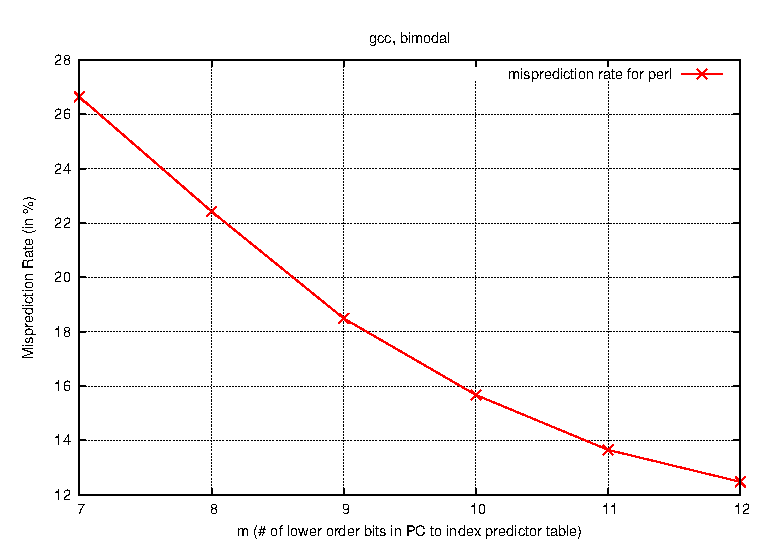
\includegraphics[scale=1.32] {image/gcc_bimodal.eps}
    \caption{Bimodal predictor misprediction rate for gcc trace}
    \label{fig:bimodal_gcc}
\end{figure}

\begin{table}[htbp]
    \centering
    \begin{tabular}{|c|c|c|c|}
        \hline
        \multirow{2}[3]{*}{\bf m (bits) } & \multicolumn{3}{c|}{\bf Misprediction Rate} \\
        \cline{2-4} & \bf gcc & \bf jpeg & \bf perl \\
        \hline
             7 & 26.65 & 7.92 & 21.31 \\
             8 & 22.43 & 7.79 & 16.45 \\
             9 & 18.49 & 7.74 & 14.14 \\
            10 & 15.67 & 7.70 & 11.95 \\
            11 & 13.65 & 7.62 & 11.05 \\
            12 & 12.47 & 7.60 &  9.09 \\
            13 & 11.72 & 7.59 &  8.92 \\
            14 & 11.37 & 7.59 &  8.82 \\
            15 & 11.30 & 7.59 &  8.82 \\
            16 & 11.21 & 7.59 &  8.82 \\
        \hline
    \end{tabular}
    \captionsetup{justification=centering}
    \caption{Experiment Data for bimodal predictor for different `m' values and traces}
    \label{tab:bimodal}
\end{table}

\begin{figure} [htbp]
    \centering
    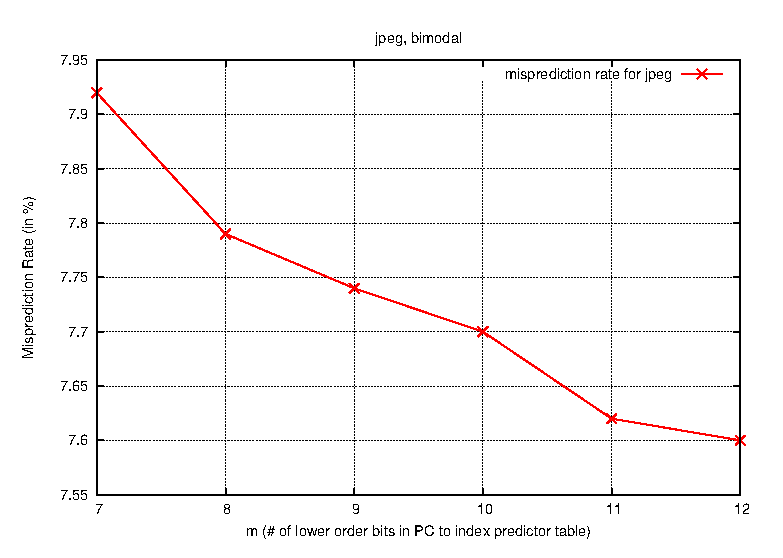
\includegraphics[scale=1.32] {image/jpeg_bimodal.eps}
    \caption{Bimodal predictor misprediction rate for jpeg trace}
    \label{fig:bimodal_jpeg}
\end{figure}

\begin{figure} [htbp]
    \centering
    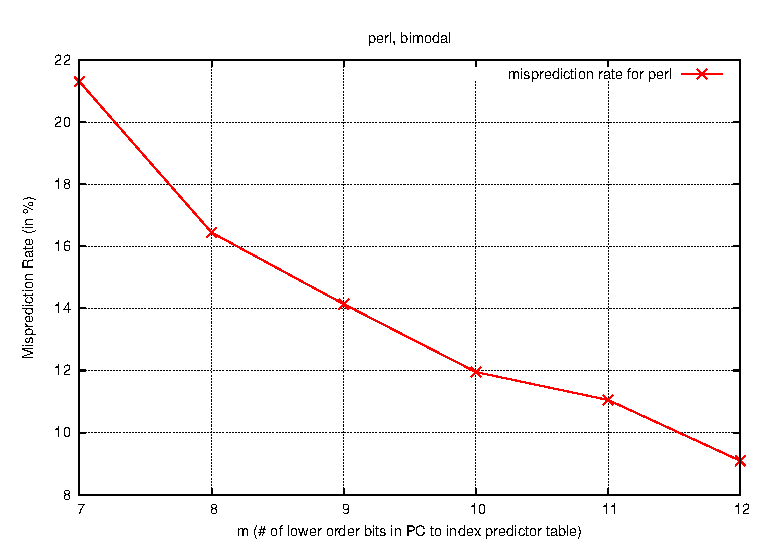
\includegraphics[scale=1.32] {image/perl_bimodal.eps}
    \caption{Bimodal predictor misprediction rate for perl trace}
    \label{fig:bimodal_perl}
\end{figure}

\subsection{Gshare Predictor Experiments}
In this experiment, the ghsare branch predictor is run against different values of m (the number of lower order bits of PC to be used as an index of the predictor table), n (the number of bits in global branch history register) and different benchmarks - gcc, jepg and perl. The misprediction rate is calculated in each case and plotted against the m value. This data is available in tables \ref{tab:gshare_gcc}, \ref{tab:gshare_jpeg} and \ref{tab:gshare_perl} and the results are plotted as graphs in figures \ref{fig:gshare_gcc}, \ref{fig:gshare_jpeg} and \ref{fig:gshare_perl}.

\begin{table}[htbp]
    \centering
    \begin{tabular}{|c|c|c|c|c|c|c|}
        \hline
        \multirow{2}[6]{*}{\bf m (bits) } & \multicolumn{6}{c|}{\bf Misprediction Rate} \\
        \cline{2-7} & \bf n = 2 & \bf n = 4 & n = 6 & \bf n = 8 & \bf n = 10 & \bf n = 12 \\
        \hline
         7 & 28.98 & 30.76 & 32.22 & - & - & - \\
         8 & 25.81 & 26.57 & 27.82 & 30.56 & - & - \\
         9 & 20.25 & 22.43 & 24.14 & 26.08 & - & - \\
        10 & 16.39 & 17.99 & 19.36 & 21.10 & 22.77 & - \\
        11 & 13.71 & 14.49 & 15.14 & 16.47 & 18.34 & - \\
        12 & 12.20 & 12.23 & 12.46 & 13.00 & 14.33 & 15.40 \\
        \hline
    \end{tabular}
    \captionsetup{justification=centering}
    \caption{Experiment Data for gshare predictor for different `m' and `n' values for gcc trace}
    \label{tab:gshare_gcc}
\end{table}

\begin{figure} [htbp]
    \centering
    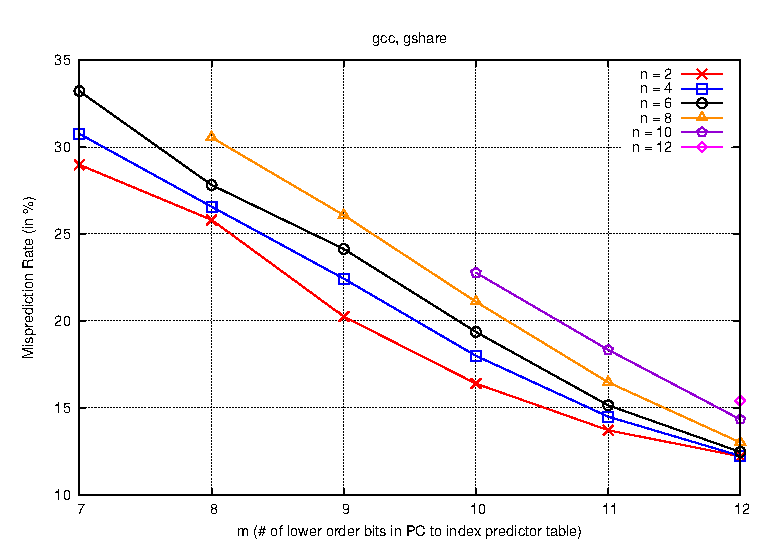
\includegraphics[scale=1.32] {image/gcc_gshare.eps}
    \caption{Ghsare predictor misprediction rate for gcc trace}
    \label{fig:gshare_gcc}
\end{figure}

\begin{table}[htbp]
    \centering
    \begin{tabular}{|c|c|c|c|c|c|c|}
        \hline
        \multirow{2}[6]{*}{\bf m (bits) } & \multicolumn{6}{c|}{\bf Misprediction Rate} \\
        \cline{2-7} & \bf n = 2 & \bf n = 4 & n = 6 & \bf n = 8 & \bf n = 10 & \bf n = 12 \\
        \hline
         7 & 8.08 & 8.92 & 9.74 & - & - & - \\
         8 & 7.79 & 7.88 & 8.87 & 9.20 & - & - \\
         9 & 7.58 & 7.68 & 8.13 & 8.30 & - & - \\
        10 & 7.49 & 7.38 & 7.58 & 7.45 & 7.95 & - \\
        11 & 7.45 & 7.27 & 7.38 & 7.17 & 7.44 & - \\
        12 & 7.44 & 7.26 & 7.19 & 6.84 & 7.18 & 7.35 \\
        \hline
    \end{tabular}
    \captionsetup{justification=centering}
    \caption{Experiment Data for gshare predictor for different `m' and `n' values for jpeg trace}
    \label{tab:gshare_jpeg}
\end{table}

\begin{figure} [htbp]
    \centering
    \includegraphics [scale=1.32] {image/jpeg_gshare.eps}
    \caption{Gshare predictor misprediction rate for jpeg trace}
    \label{fig:gshare_jpeg}
\end{figure}

\begin{table}[htbp]
    \centering
    \begin{tabular}{|c|c|c|c|c|c|c|}
        \hline
        \multirow{2}[6]{*}{\bf m (bits) } & \multicolumn{6}{c|}{\bf Misprediction Rate} \\
        \cline{2-7} & \bf n = 2 & \bf n = 4 & n = 6 & \bf n = 8 & \bf n = 10 & \bf n = 12 \\
        \hline
         7 & 24.34 & 25.96 & 28.71 &     - &     - &    - \\
         8 & 16.92 & 19.09 & 20.45 & 24.79 &     - &    - \\
         9 & 13.57 & 14.68 & 16.25 & 17.66 &     - &    - \\
        10 & 10.63 & 11.35 & 11.52 & 12.42 & 14.57 &    - \\
        11 & 10.11 &  9.68 &  8.60 &  9.00 &  8.98 &    - \\
        12 &  9.04 &  8.09 &  7.50 &  6.49 &  6.71 & 7.16 \\
        \hline
    \end{tabular}
    \captionsetup{justification=centering}
    \caption{Experiment Data for gshare predictor for different `m' and `n' values for perl trace}
    \label{tab:gshare_perl}
\end{table}

\begin{figure} [htbp]
    \centering
    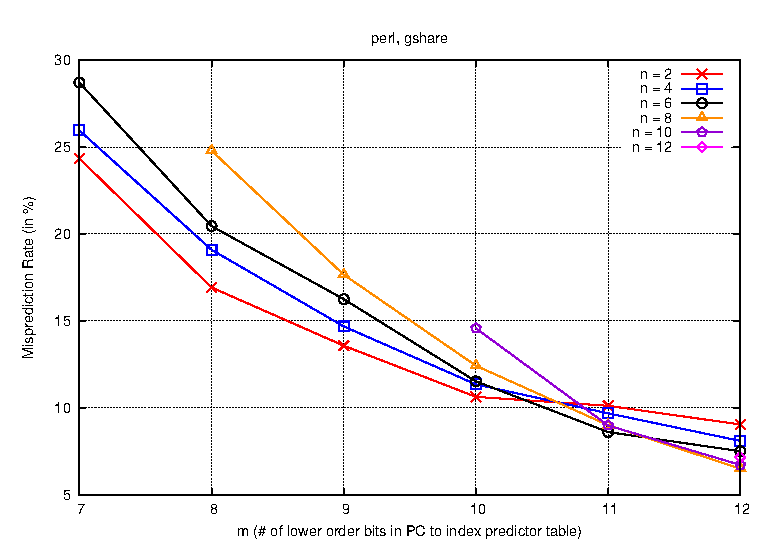
\includegraphics [scale=1.32] {image/perl_gshare.eps}
    \caption{Gshare predictor misprediction rate for perl trace}
    \label{fig:gshare_perl}
\end{figure}

